In this Chapter we give an overview of functionality contained in the {\tt amrex/Src/AmrCore} source code.
This directory contains source code for the following:
\begin{itemize}
\item Storing information about the grid layout and processor distribution mapping
at each level of refinement.
\item Functions to create grids at different levels of refinement, including tagging
operationrs.
\item Operations on data at different levels of refinement, such as interpolation and
restriction operators.
\item Flux registers used to store and manipulate fluxes at coarse-fine interfaces.
\item Particle support for AMR (see Chapter\ref{Chap:Particles}).
\end{itemize}
There is another source directory, {\tt amrex/Src/Amr/}, which contains
additional classes used to manage the time-stepping for AMR simulations.
However, it is possible to build a fully adaptive, subcycling-in-time simulation code
without these additional classes.

In this Chapter, we restrict our use to the {\tt amrex/Src/AmrCore} source code
and present a tutorial that performs an adaptive, subcycling-in-time simulation
of the advection equation for a passively advected scalar.
The accompanying tutorial code is available in {\tt amrex/Tutorials/Amr/Advection\_AmrCore}
with build/run directory {\tt Exec/SingleVortex}.  In this example, the velocity
field is a specified function of space and time, such that an initial
Gaussian profile is displaced but returns to its original configuration at the final time.
The boundary conditions are periodic and we use a refinement ratio of $r=2$ between each 
AMR level.  The results of the simulation in two-dimensions are depicted in 
Figure \ref{fig:Adv}.
%%%%%%%%%%%%%%%%%%%%%%%%%%%%%
\begin{figure}
  \centering
  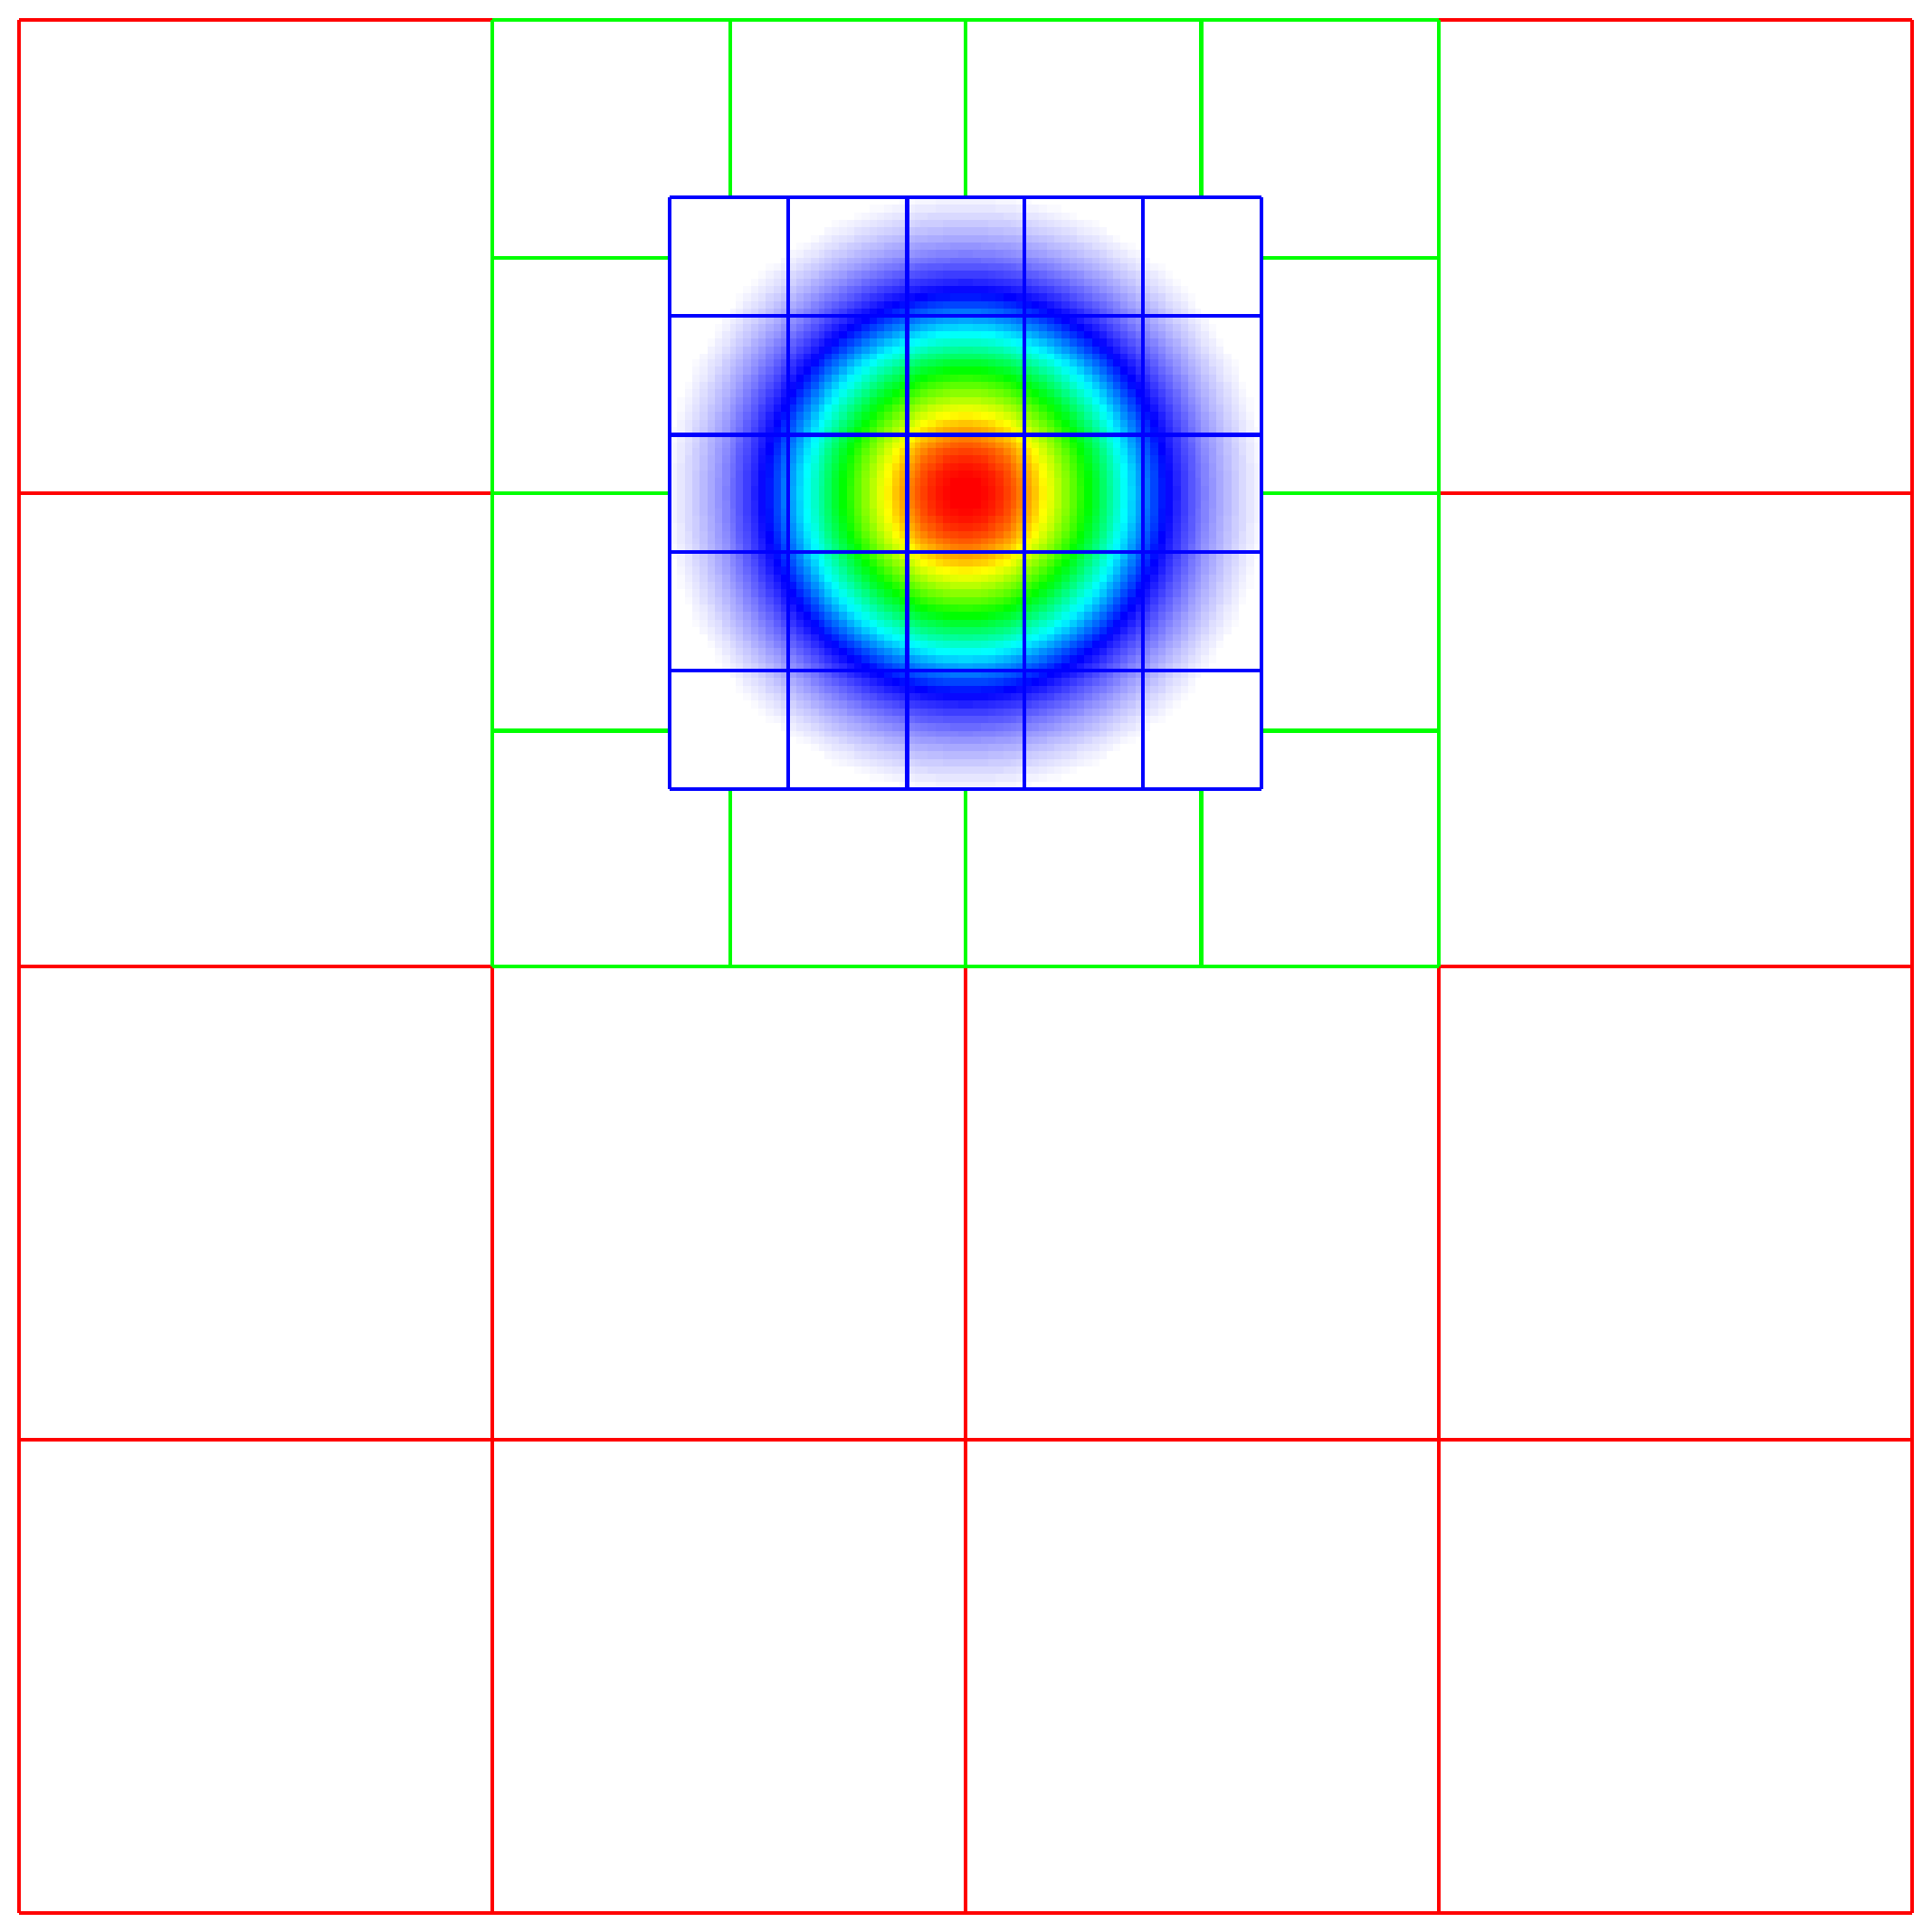
\includegraphics[width=1in]{./AmrCore/figs/Adv1.pdf}
  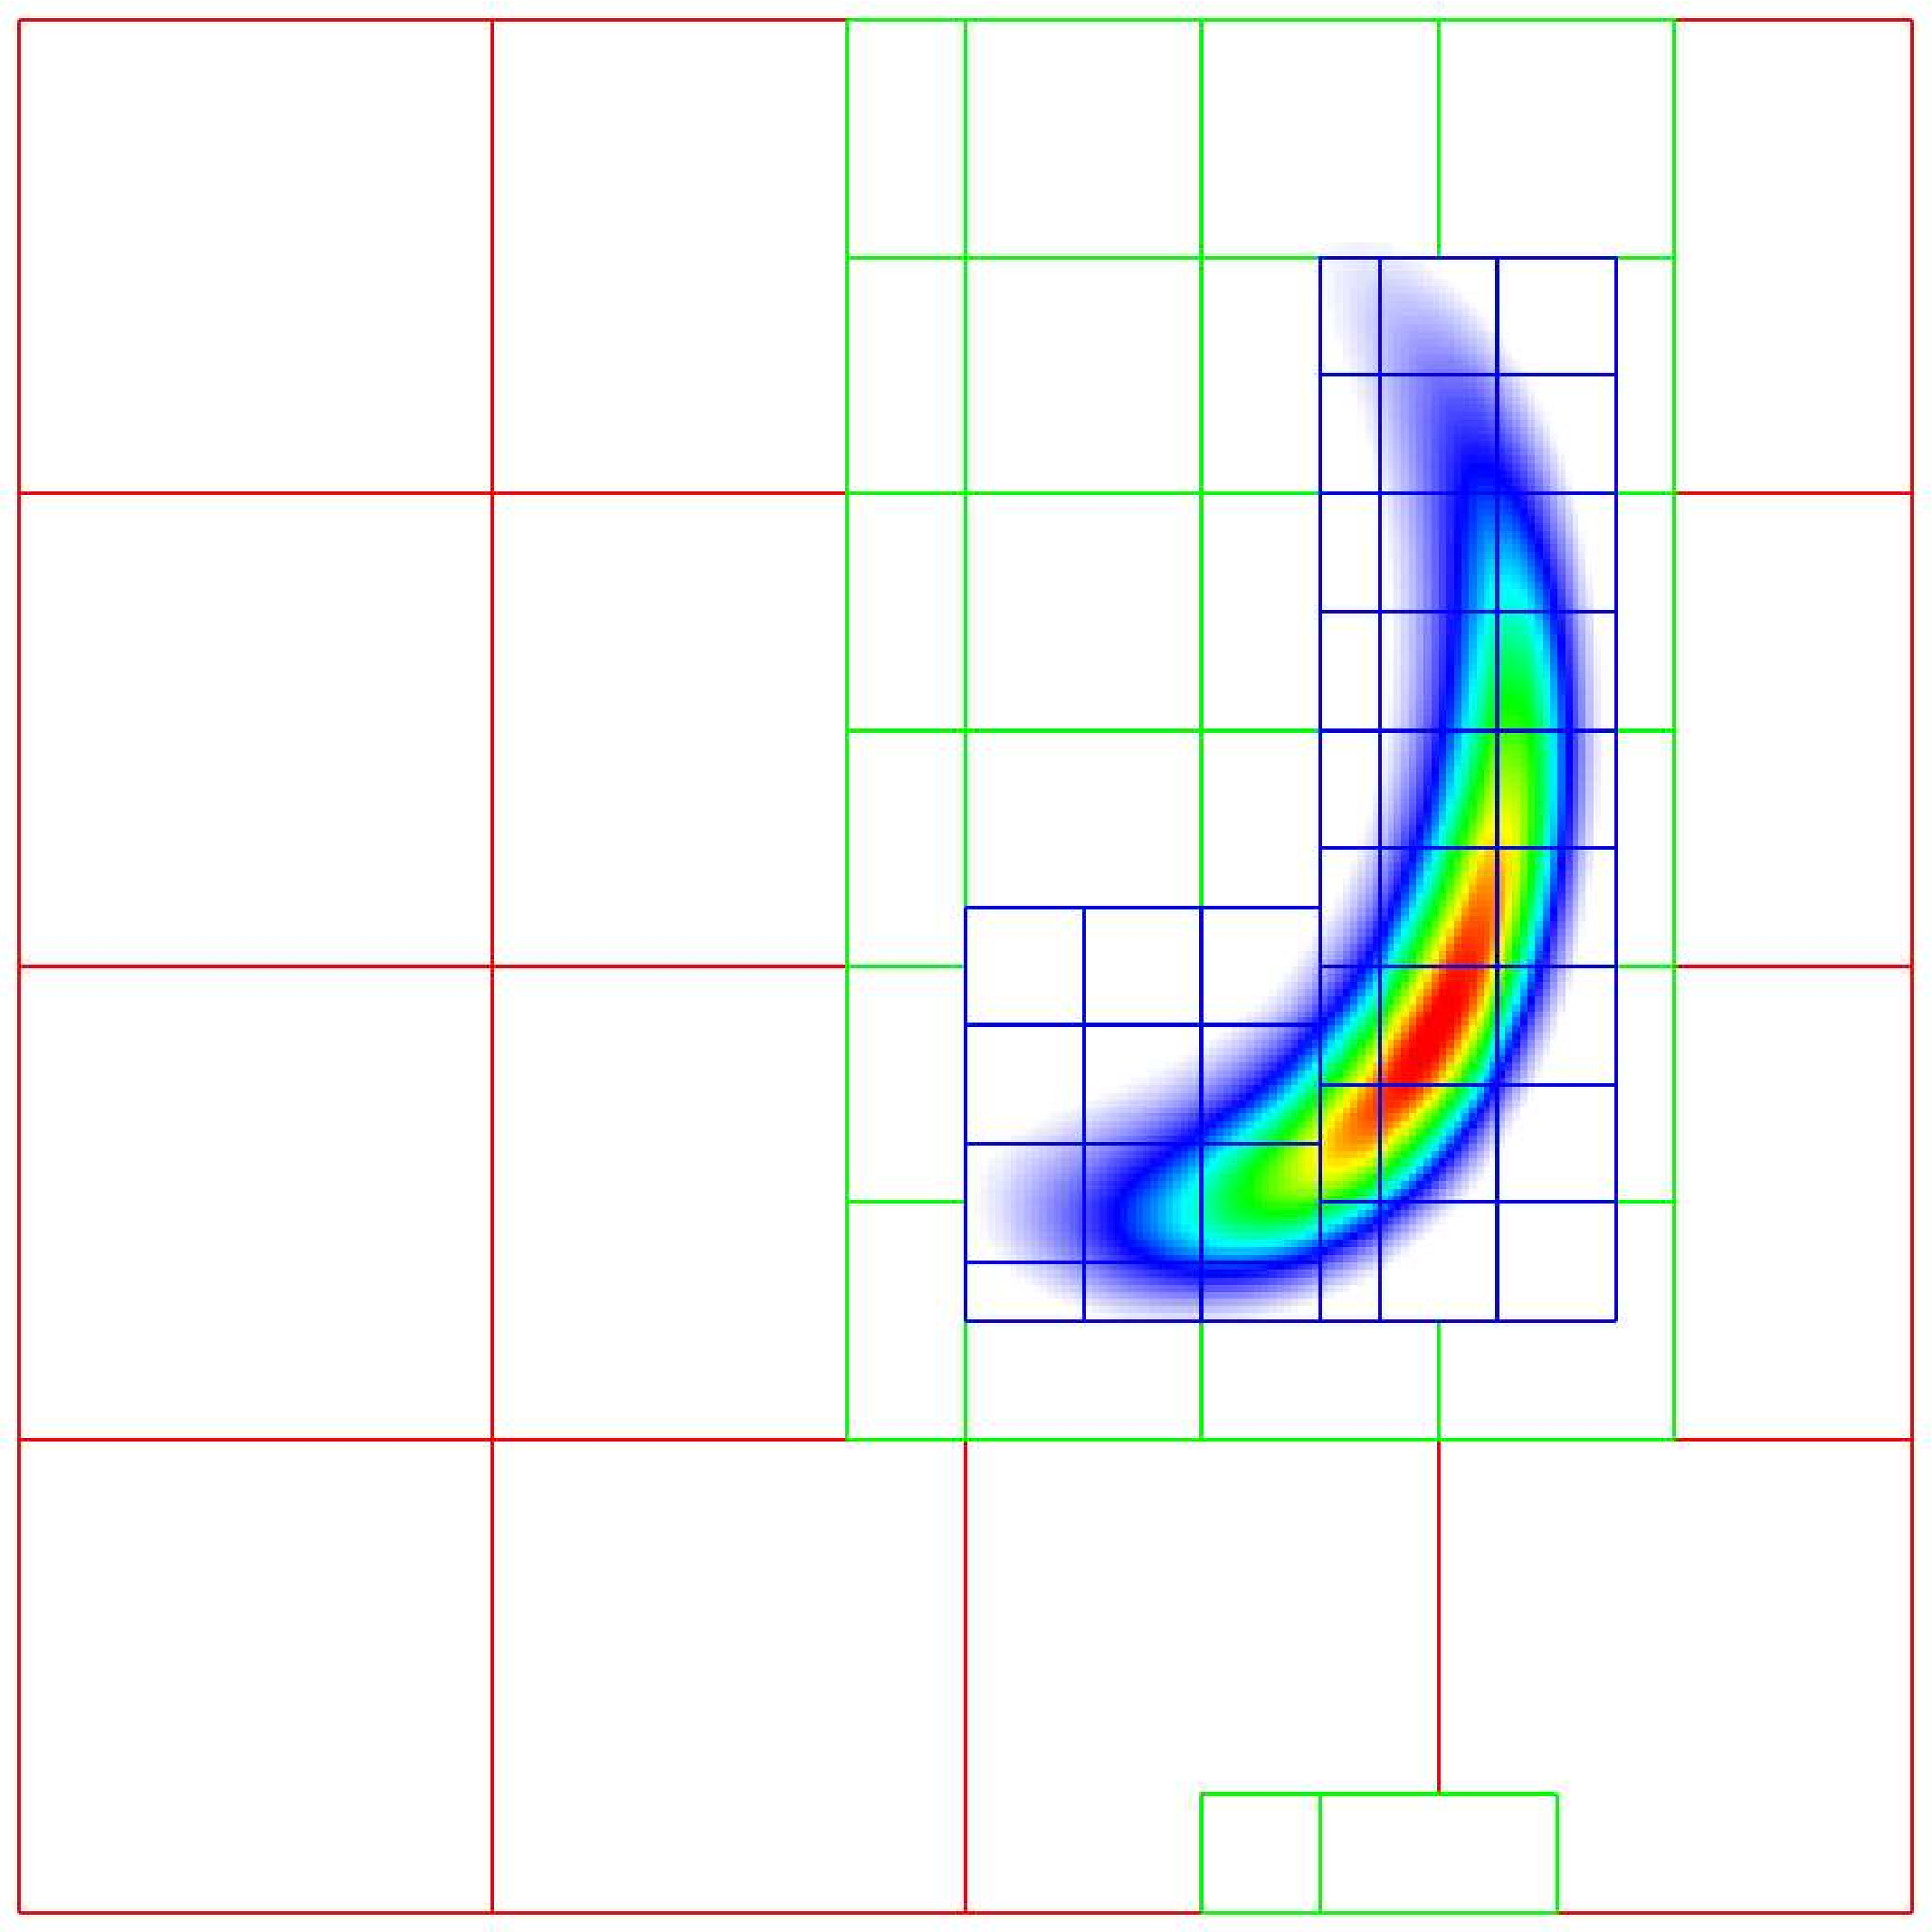
\includegraphics[width=1in]{./AmrCore/figs/Adv2.pdf}
  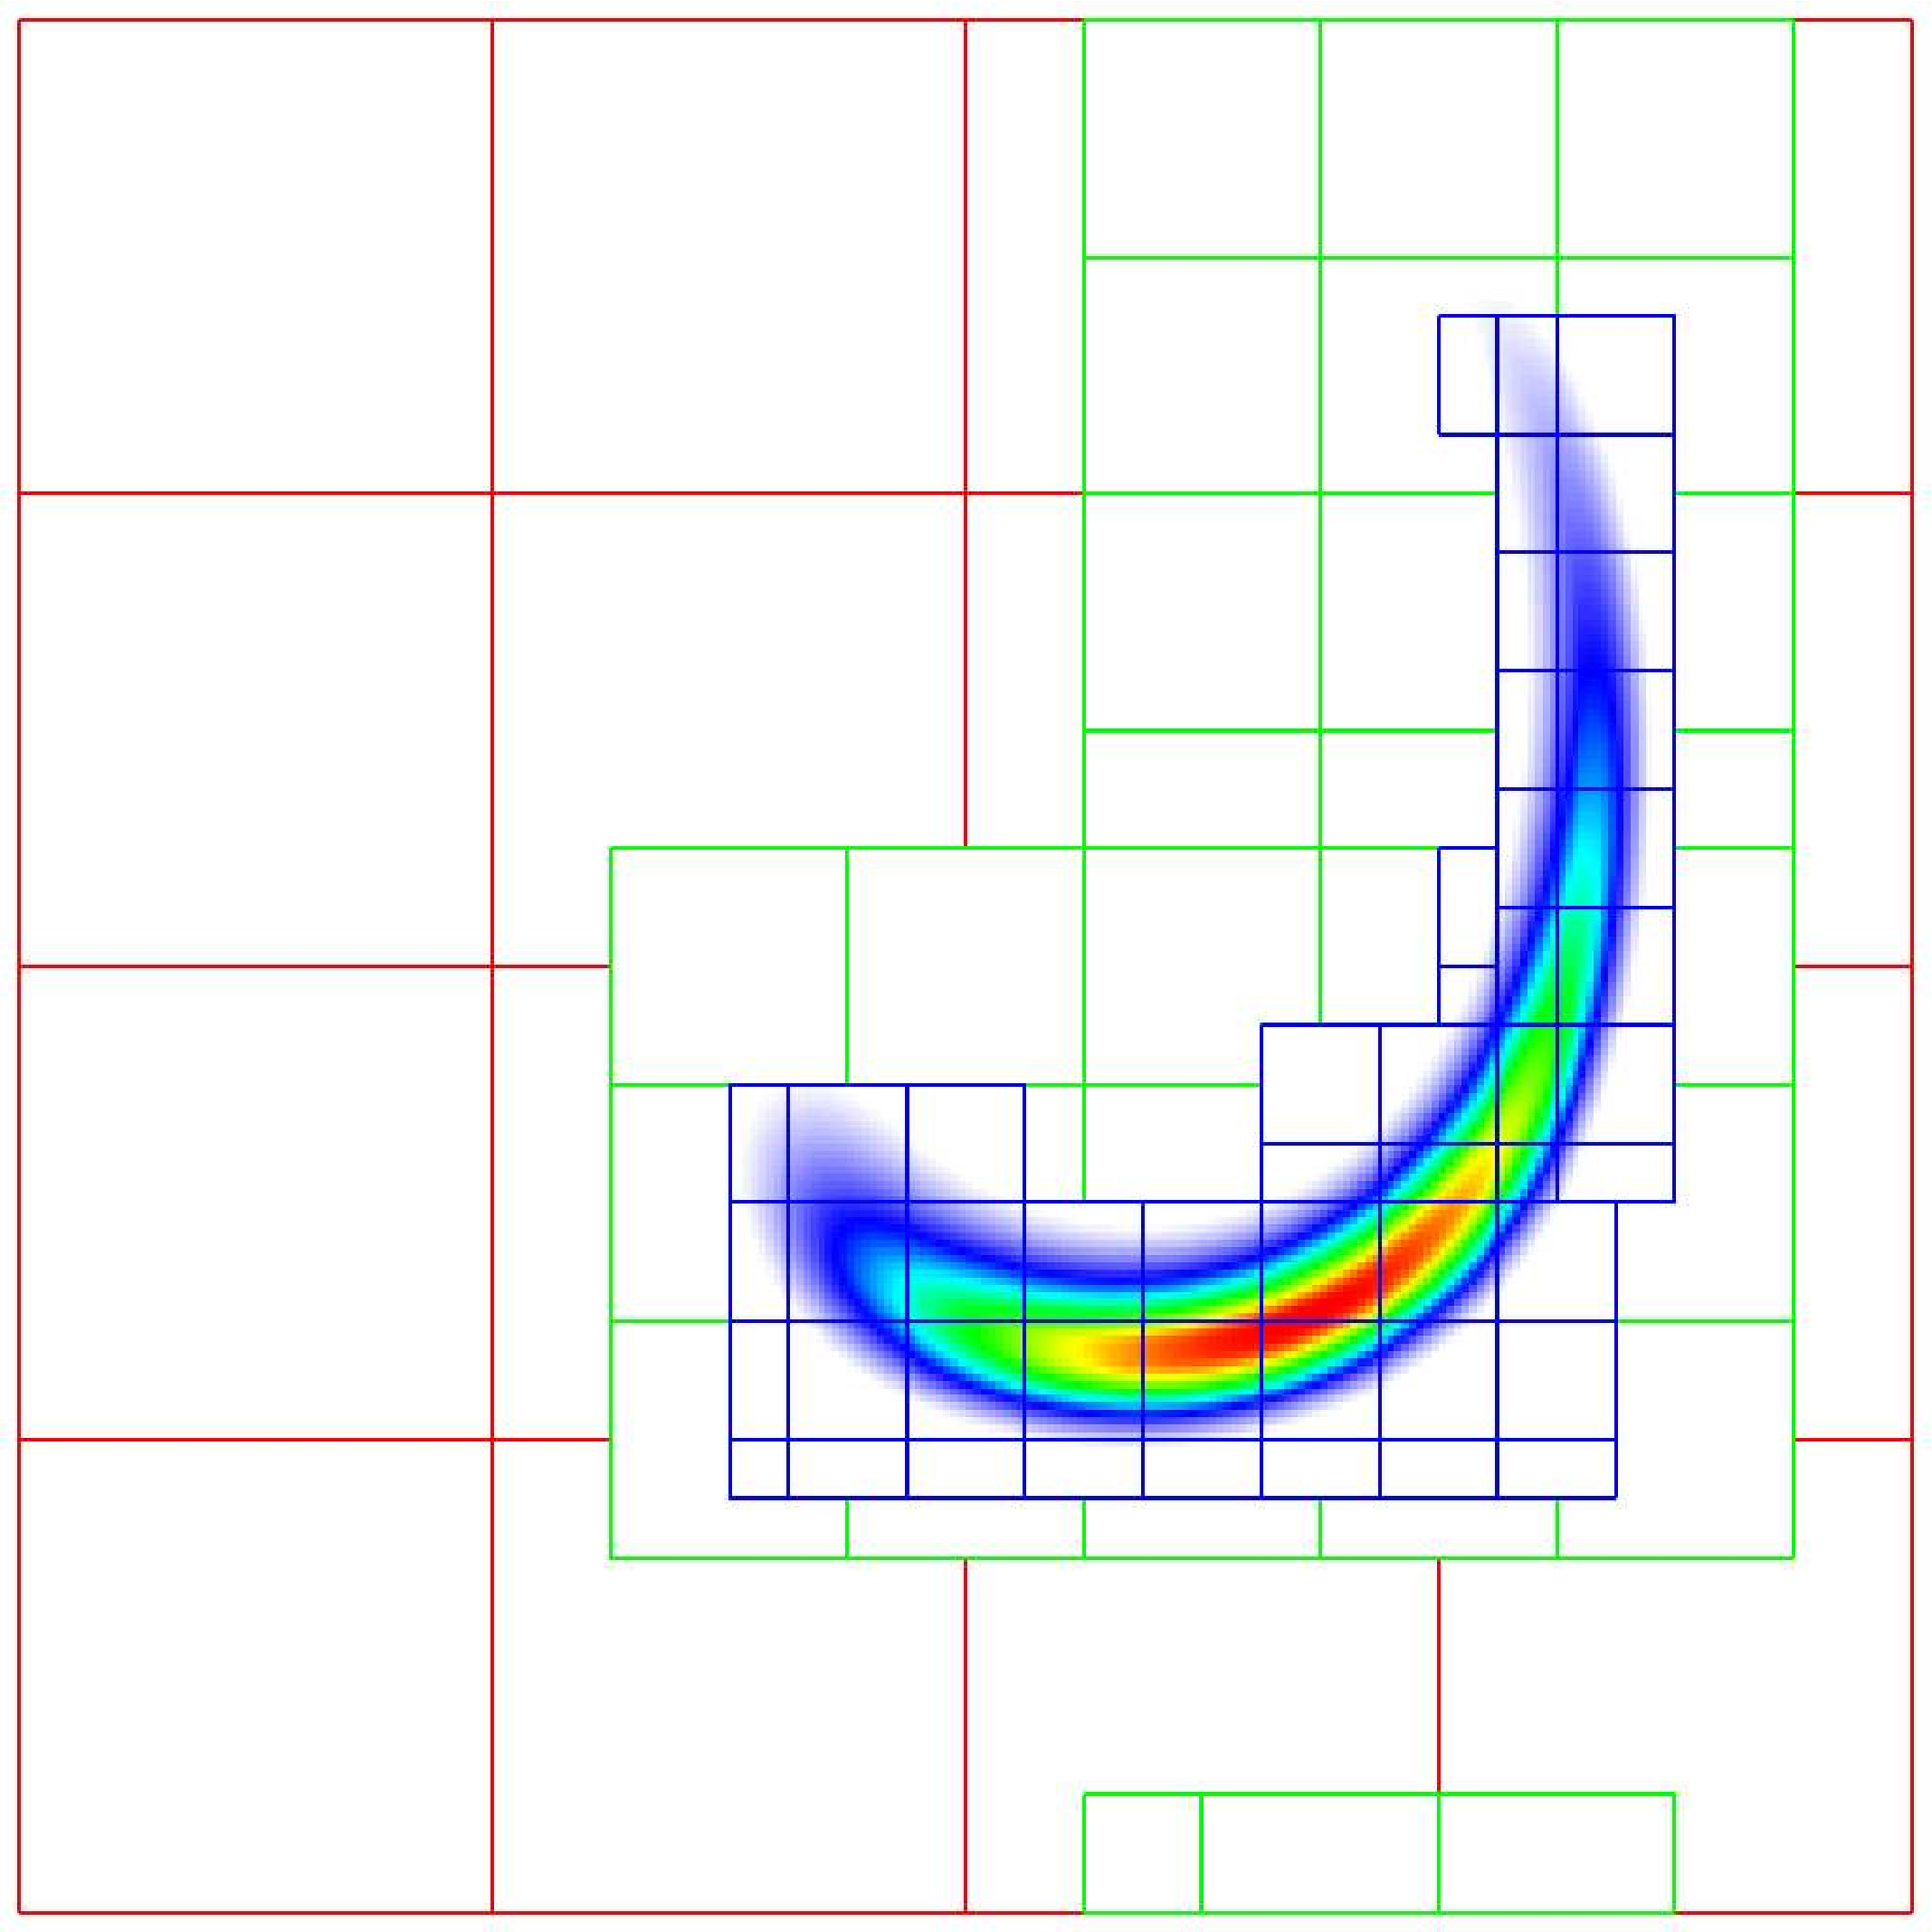
\includegraphics[width=1in]{./AmrCore/figs/Adv3.pdf}
  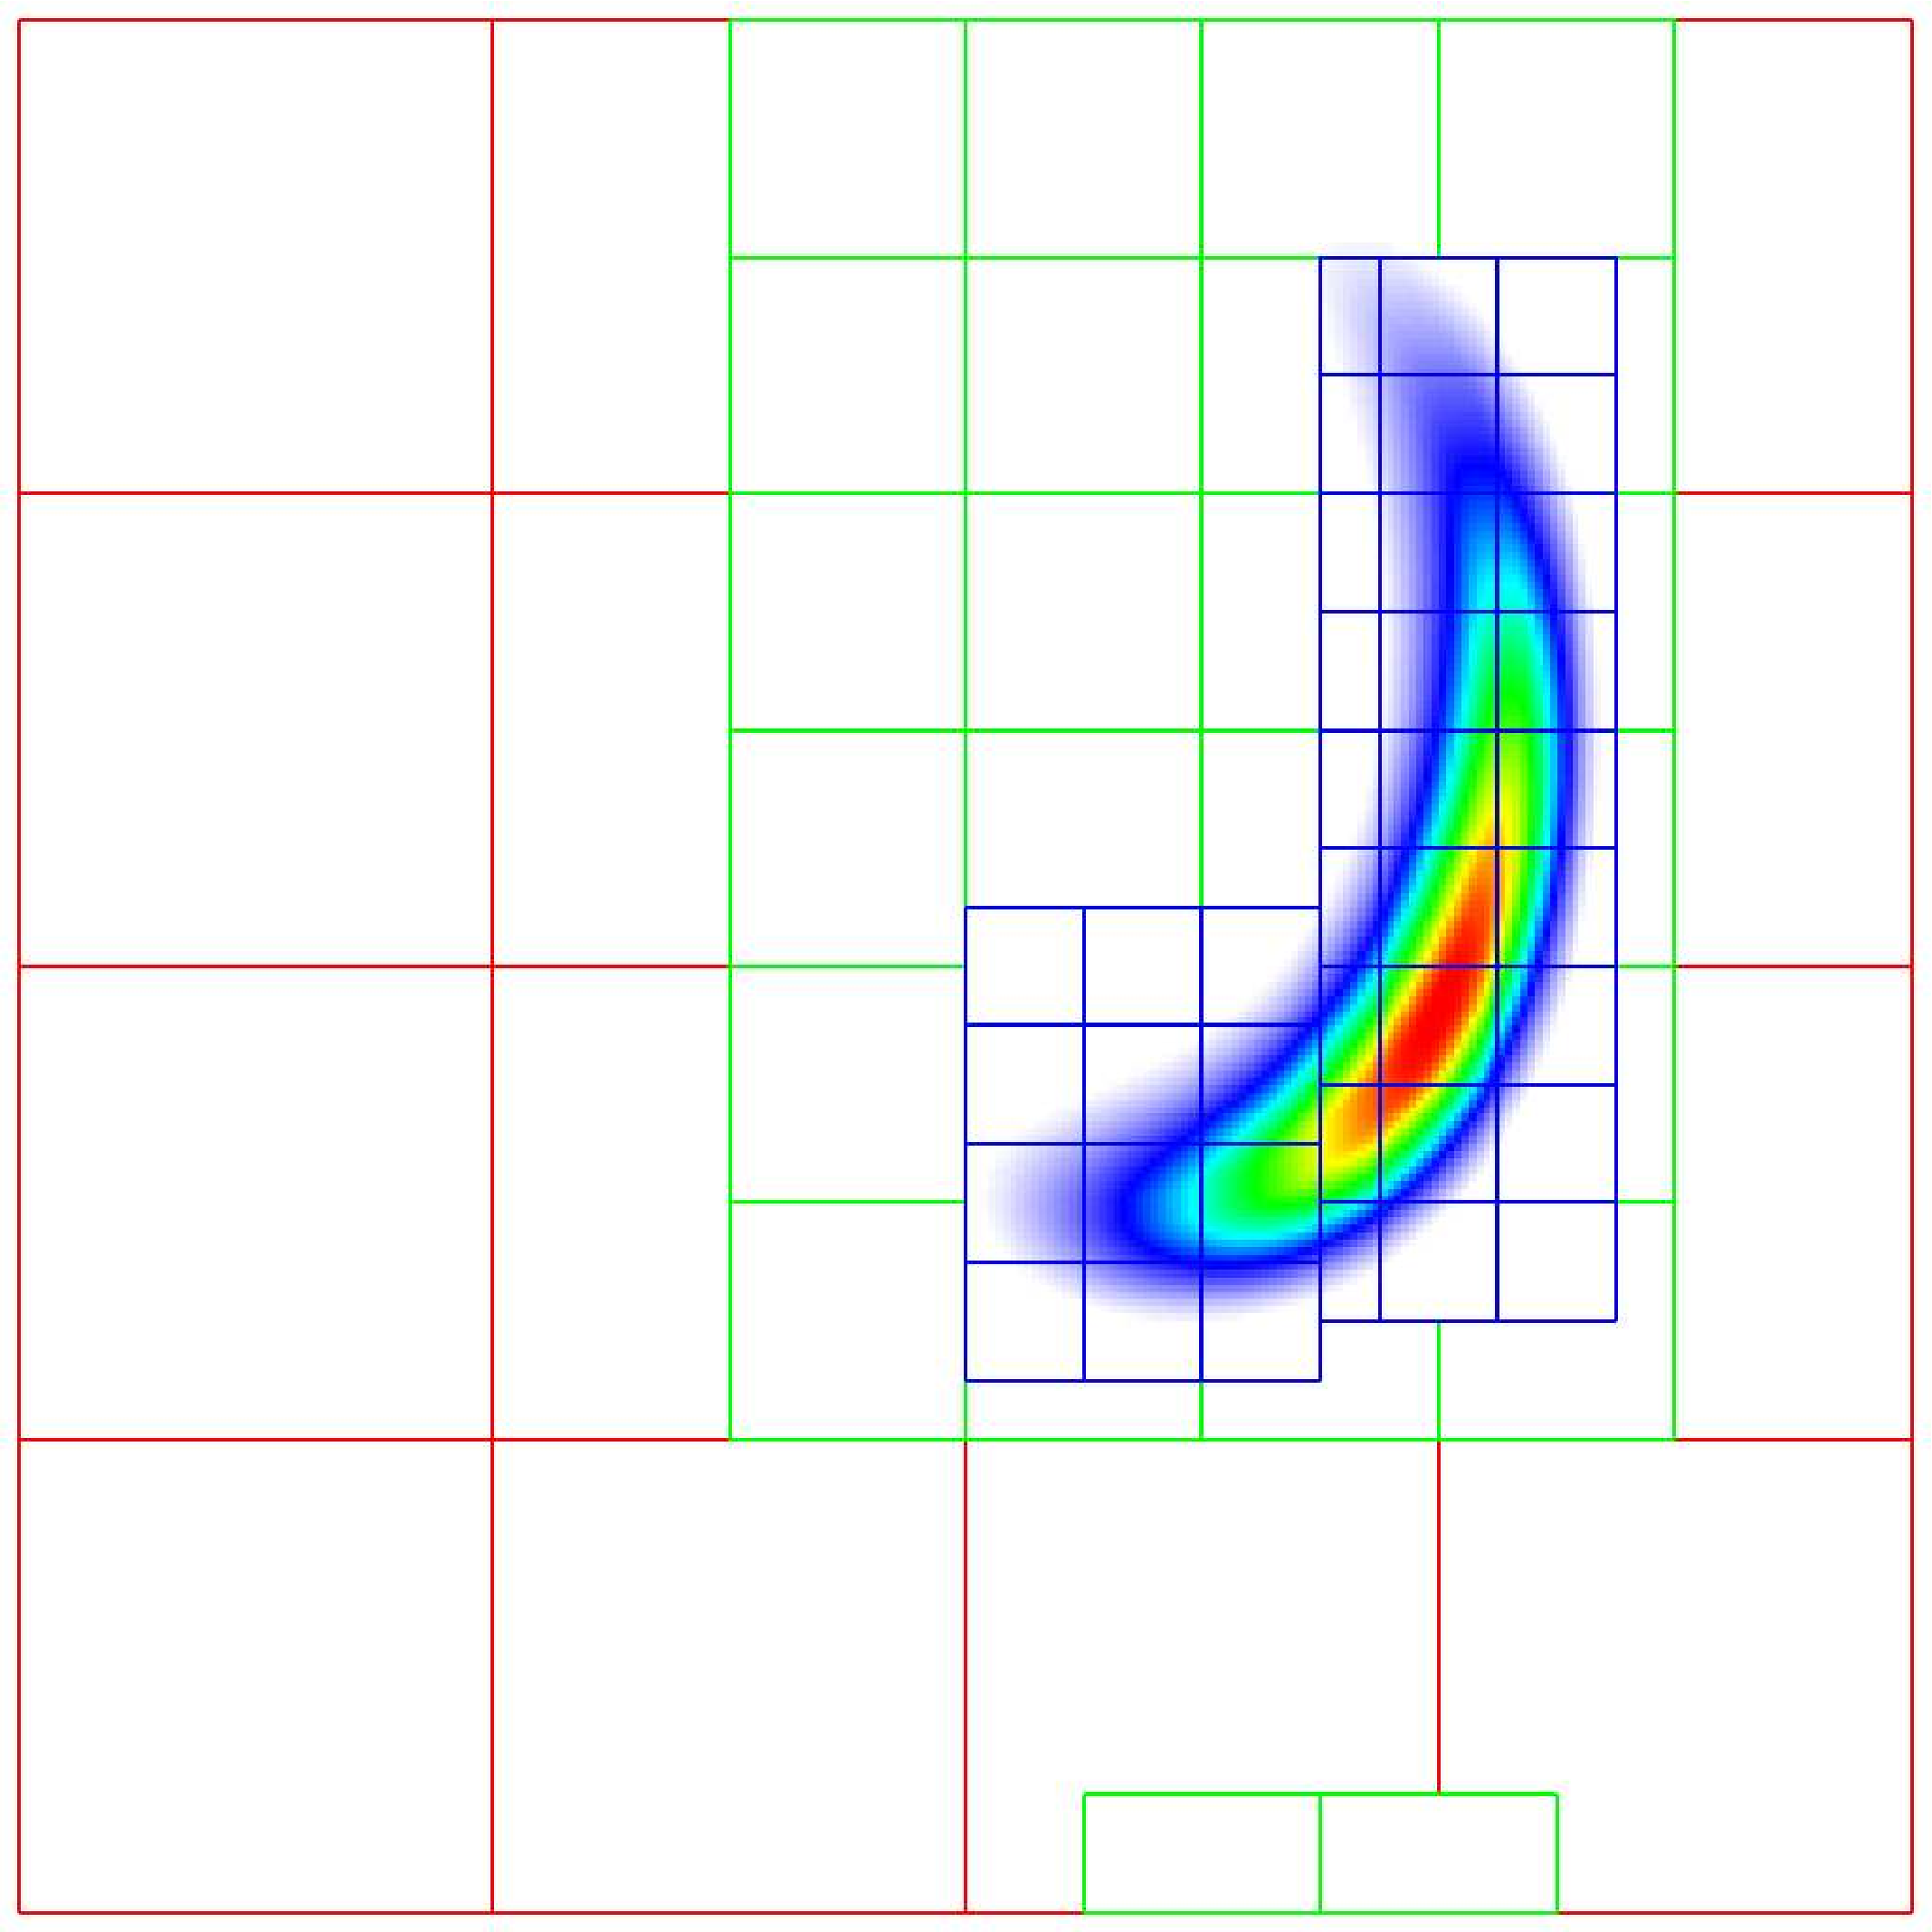
\includegraphics[width=1in]{./AmrCore/figs/Adv4.pdf}
  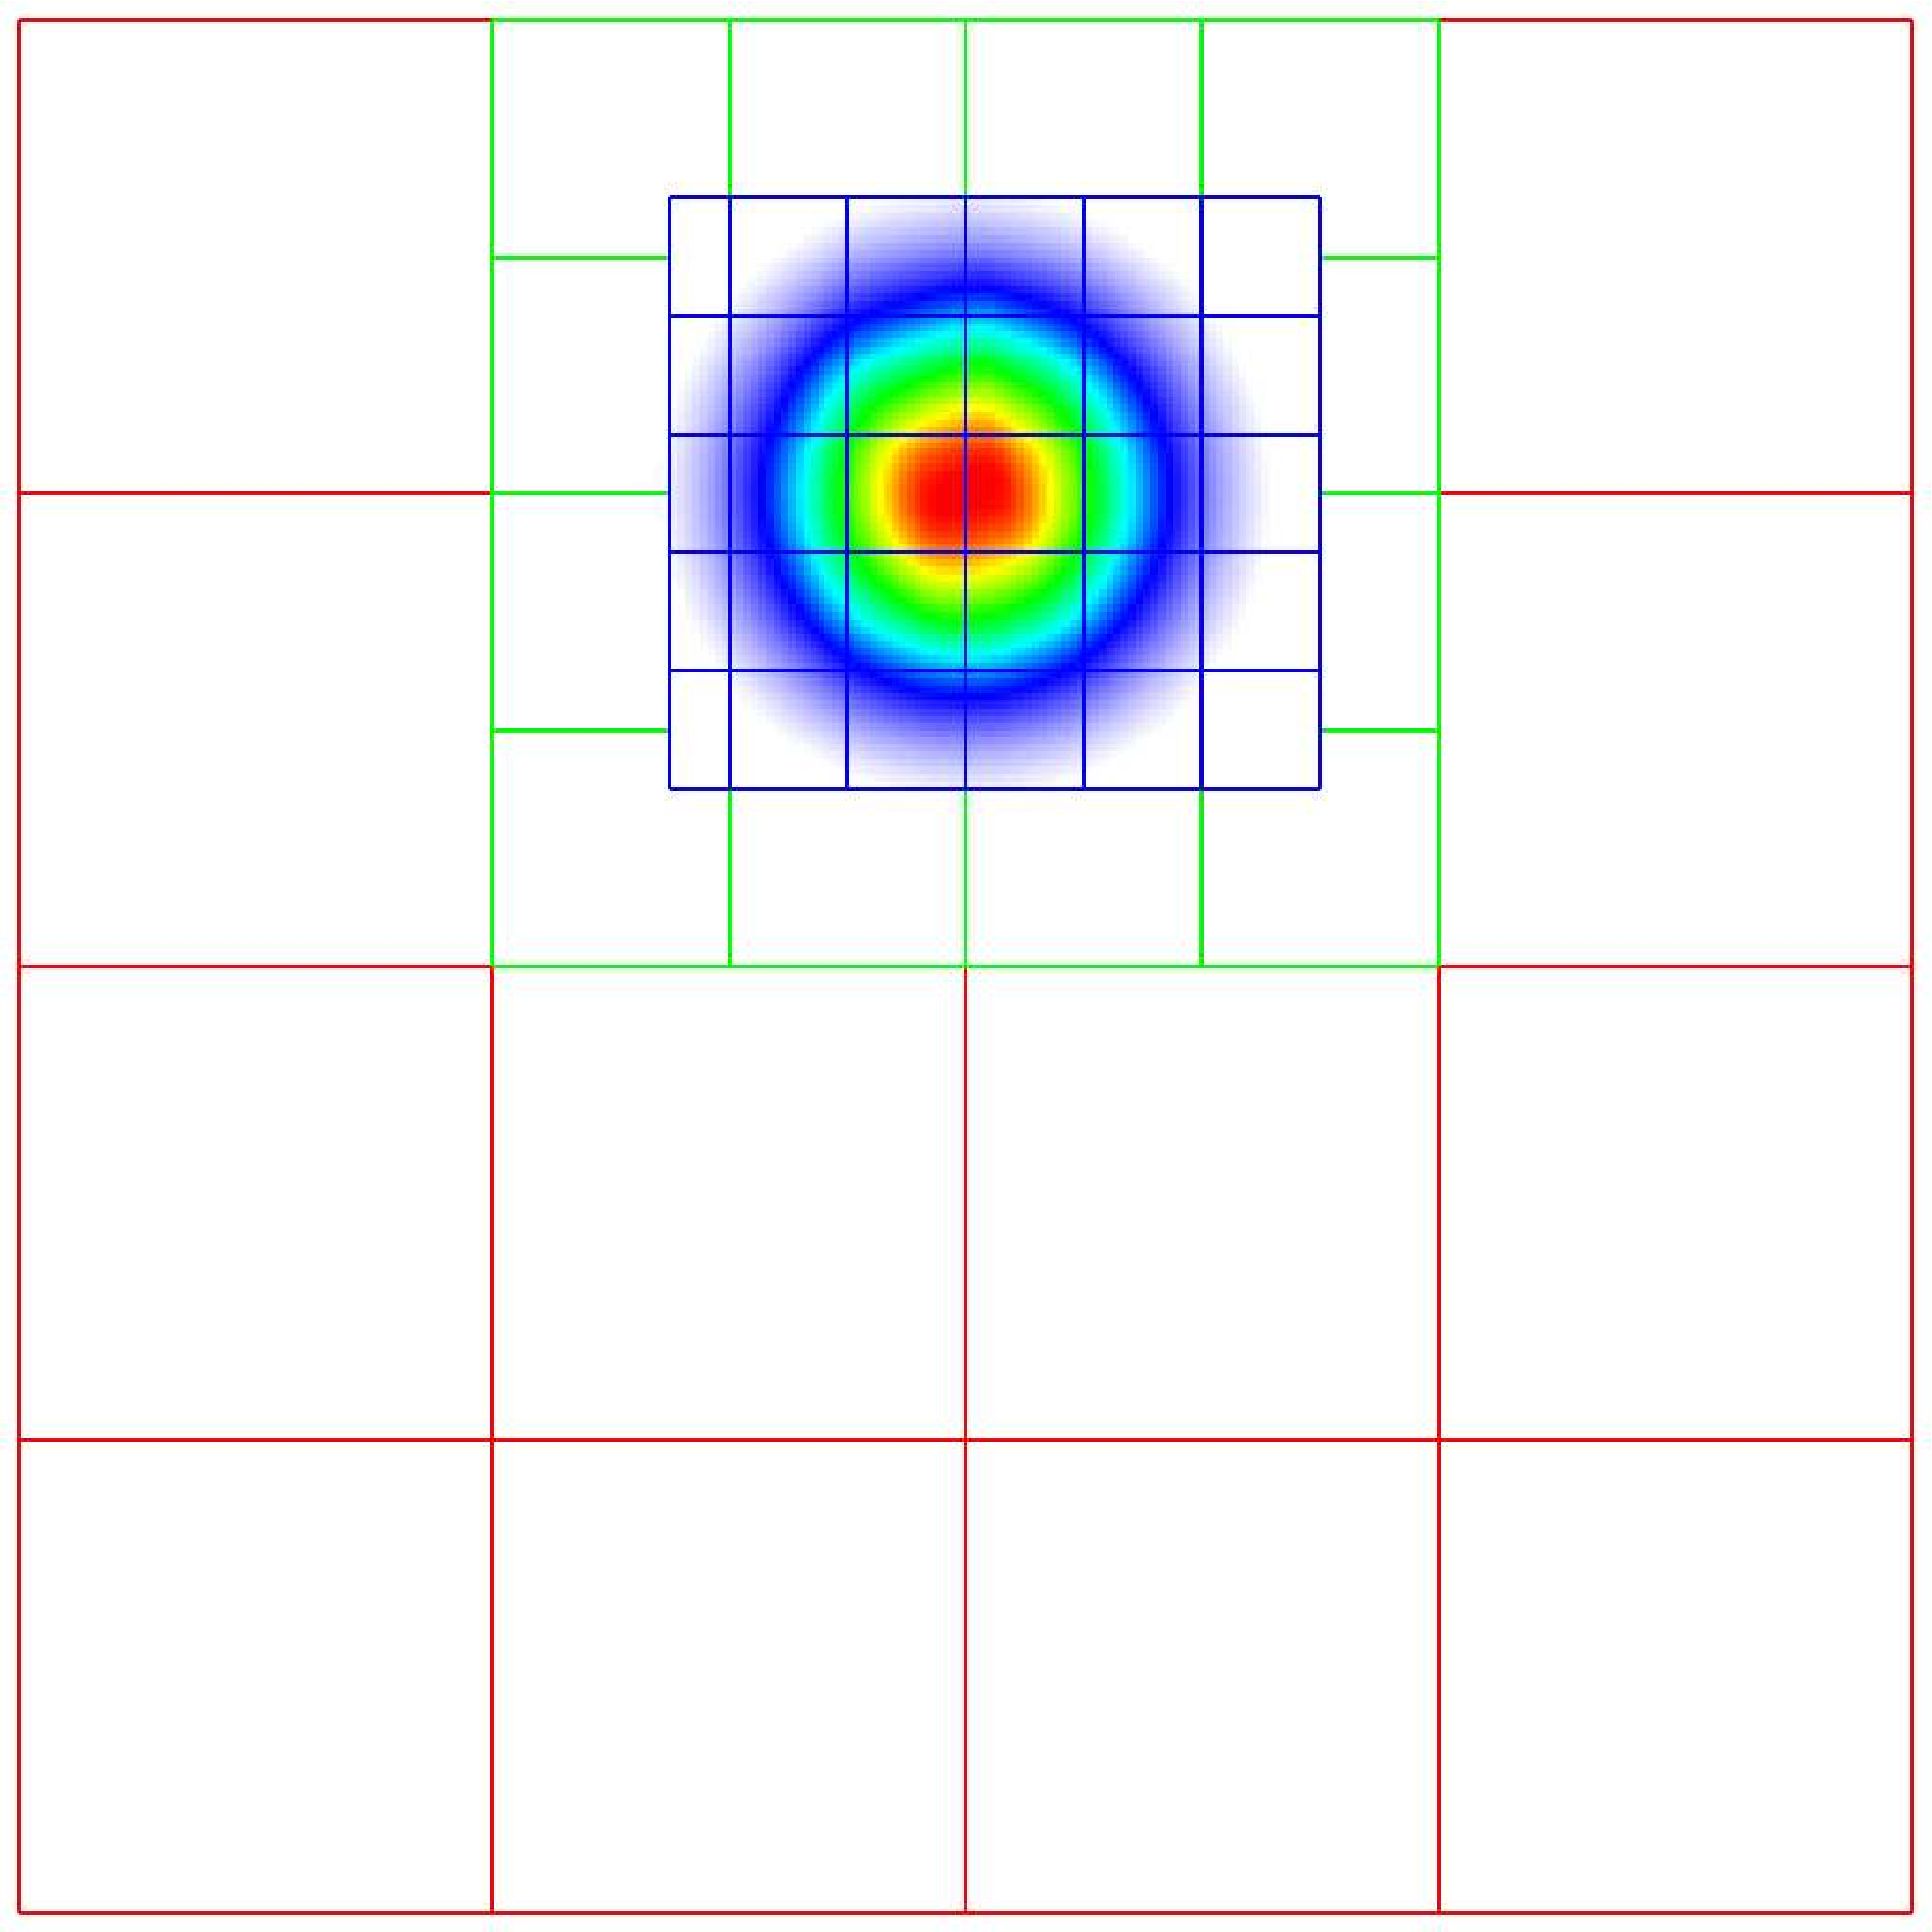
\includegraphics[width=1in]{./AmrCore/figs/Adv5.pdf}
  \caption{\label{fig:Adv} Time sequence ($t=0,0.5,1,1.5,2$~s) of advection of a Gaussian profile using the 
{\tt SingleVortex} tutorial.  The red, green, and blue boxes indicate grids at AMR levels $\ell=0,1$, and $2$.}
\end{figure}
%%%%%%%%%%%%%%%%%%%%%%%%%%%%%

\section{The Advection Equation}
We seek to solve the advection equation on a multi-level, adaptive grid structure:
\begin{equation}
\frac{\partial\phi}{\partial t} = -\nabla\cdot(\phi{\bf U}).
\end{equation}
The velocity field is a specified divergence-free (so the flow field is incompressible)
function of space and time.  The initial scalar field is a
Gaussian profile.  To integrate these equations on a given level, we use a simple conservative update,
\begin{equation}
\frac{\phi_{i,j}^{n+1}-\phi_{i,j}^n}{\Delta t} = \frac{(\phi u)_{i+\myhalf,j}^{n+\myhalf}-(\phi u)_{i-\myhalf,j}^{n+\myhalf}}{\Delta x} + \frac{(\phi v)_{i,j+\myhalf}^{n+\myhalf} - (\phi v)_{i,j-\myhalf}^{n+\myhalf}}{\Delta y},
\end{equation}
where the velocities on faces are prescribed functions of space and time, and the scalars on faces
are computed using a Godunov advection integration scheme.  The fluxes in this case are the face-centered,
time-centered ``$\phi u$'' and ``$\phi v$'' terms.

We use a subcycling-in-time approach where finer levels are advanced with smaller
time steps than coarser levels, and then synchronization is later performed between levels.
More specifically, the multi-level procedure can most
easily be thought of as a recursive algorithm in which, to advance level $\ell$,
$0\le\ell\le\ell_{\rm max}$, the following steps are taken:
\begin{itemize}
\item Advance level $\ell$ in time by one time step, $\Delta t^{\ell}$, as if it is
the only level.  If $\ell>0$, obtain boundary data (i.e. fill the level $\ell$ ghost cells)
using space- and time-interpolated data from the grids at $\ell-1$ where appropriate.
\item If $\ell<\ell_{\rm max}$
\begin{itemize}
\item Advance level $(\ell+1)$ for $r$ time steps with $\Delta t^{\ell+1} = \frac{1}{r}\Delta t^{\ell}$.
\item Synchronize the data between levels $\ell$ and $\ell+1$.
\end{itemize}
\end{itemize}
Specifically, for a 3-level simulation, depicted graphically in Figure \ref{fig:subcycling}:
\begin{enumerate}
\item Integrate $\ell=0$ over $\Delta t$.
\item Integrate $\ell=1$ over $\Delta t/2$.
\item Integrate $\ell=2$ over $\Delta t/4$.
\item Integrate $\ell=2$ over $\Delta t/4$.
\item Synchronize levels $\ell=1,2$.
\item Integrate $\ell=1$ over $\Delta t/2$.
\item Integrate $\ell=2$ over $\Delta t/4$.
\item Integrate $\ell=2$ over $\Delta t/4$.
\item Synchronize levels $\ell=1,2$.
\item Synchronize levels $\ell=0,1$.
\end{enumerate}
%%%%%%%%%%%%%%%%%%%%%%%%%%%%%
\begin{figure}[htb]
\begin{center}
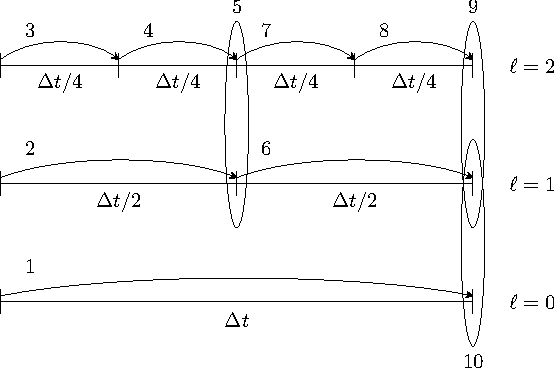
\includegraphics[width=4in]{./AmrCore/figs/subcycling.pdf}
\caption{\label{fig:subcycling} Schematic of subcycling-in-time algorithm.}
\end{center}
\end{figure}
%%%%%%%%%%%%%%%%%%%%%%%%%%%%%
For the scalar field, we keep track volume and time-weighted fluxes at coarse-fine interfaces.
We accumulate area and time-weighted fluxes in {\tt FluxRegister} objects, which can be
thought of as special boundary {\tt FABset}s associated with coarse-fine interfaces.
Since the fluxes are area and time-weighted (and sign-weighted, depending on whether they
come from the coarse or fine level), the flux registers essentially store the extent by
which the solution does not maintain conservation.  Conservation only happens if the
sum of the (area and time-weighted) fine fluxes equals the coarse flux, which in general 
is not true.

The idea behind the level $\ell/(\ell+1)$ synchronization step is to correct for sources of 
mismatch in the composite solution:
\begin{enumerate}
\item The data at level $\ell$ that underlie the level  $\ell+1$ data are not synchronized with the level $\ell+1$ data.
This is simply corrected by overwriting covered coarse cells to be the average of the overlying fine cells.
\item The area and time-weighted fluxes from the level $\ell$ faces and the level $\ell+1$ faces
do not agree at the $\ell/(\ell+1)$ interface, resulting in a loss of conservation.  
The remedy is to modify the solution in the coarse cells immediately next to the coarse-fine interface
to account for the mismatch stored in the flux register (computed by taking the coarse-level divergence of the
flux register data).
\end{enumerate}

\section{{\tt AmrCore} Source Code}
Here we provide a high-level overview of the source code in {\tt amrex/Src/AmrCore}.

\subsection{{\tt AmrMesh} and {\tt AmrCore}}

For single-level simulations
(see e.g., {\tt amrex/Tutorials/Basic/HeatEquation\_EX1\_C/main.cpp})
the user needs to build {\tt Geometry}, {\tt DistributionMapping},
and {\tt BoxArray} objects associated with the simulation.  For simulations
with multiple levels of refinement, the {\tt AmrMesh} class can be thought
of as a container to store arrays of these objects (one for each level), and
information about the current grid structure.

{\tt amrex/Src/AmrCore/AMReX\_AmrMesh.cpp/H} contains the {\tt AmrMesh} class.
The protected data members are:
\begin{lstlisting}[language=cpp]
protected:
    int            verbose;
    int            max_level;       // Maximum allowed level.
    Array<IntVect> ref_ratio;       // Refinement ratios [0:finest_level-1]

    int            finest_level;    // Current finest level.

    Array<int>     n_error_buf;     // Buffer cells around each tagged cell.
    Array<int>     blocking_factor; // Blocking factor in grid generation 
                                    // (by level).
    Array<int>     max_grid_size;   // Maximum allowable grid size (by level).
    Real           grid_eff;        // Grid efficiency.
    int            n_proper;        // # cells required for proper nesting.

    bool use_fixed_coarse_grids;
    int  use_fixed_upto_level;
    bool refine_grid_layout;        // chop up grids to have the number of 
                                    // grids no less the number of procs

    Array<Geometry>            geom;
    Array<DistributionMapping> dmap;
    Array<BoxArray>            grids;    
\end{lstlisting}

{\tt AMReX\_AmrCore.cpp/H} contains the pure virtual class {\tt AmrCore}, 
which is derived from the {\tt AmrMesh} class.  {\tt AmrCore} does not actually 
have any data members, just additional member functions, some of which override 
the base class {\tt AmrMesh}.

There are no pure virutal functions in {\tt AmrMesh}, but 
there are 5 pure virtual functions in the {\tt AmrCore} class.  Any applications
you create must implement these functions.  The tutorial code 
{\tt Amr/Advection\_AmrCore} provides sample implementation in the derived
class {\tt AmrCoreAdv}.

\begin{lstlisting}[language=cpp]
//! Tag cells for refinement.  TagBoxArray tags is built on level lev grids.
virtual void ErrorEst (int lev, TagBoxArray& tags, Real time, 
                       int ngrow) override = 0;

//! Make a new level from scratch using provided BoxArray and DistributionMapping.
//! Only used during initialization.
virtual void MakeNewLevelFromScratch (int lev, Real time, const BoxArray& ba, 
                                      const DistributionMapping& dm) override = 0;

//! Make a new level using provided BoxArray and DistributionMapping and fill 
//  with interpolated coarse level data.
virtual void MakeNewLevelFromCoarse (int lev, Real time, const BoxArray& ba, 
                                     const DistributionMapping& dm) = 0;

//! Remake an existing level using provided BoxArray and DistributionMapping 
//  and fill with existing fine and coarse data.
virtual void RemakeLevel (int lev, Real time, const BoxArray& ba, 
                          const DistributionMapping& dm) = 0;

//! Delete level data
virtual void ClearLevel (int lev) = 0;
\end{lstlisting}
Refer to the {\tt AmrCoreAdv} class in the 
{\tt amrex/Tutorials/Amr/AmrCore\_Advection/Source} 
code for a sample implementation.

\subsection{{\tt TagBox}, and {\tt Cluster}}
These classes are used in the grid generation process.
The {\tt TagBox} class is essentially a data structure that marks which
cells are ``tagged'' for refinement.
{\tt Cluster} (and {\tt ClusterList} contained within the same file) are classes
that help sort tagged cells and generate a grid structure that contains all
the tagged cells.  These classes and their member functions are largely
hidden from any application codes through simple interfaces
such as {\tt regrid} and {\tt ErrorEst} (a routine for tagging cells for refinement).

\subsection{{\tt FillPatchUtil} and {\tt Interpolater}}\label{sec:amrcore:fillpatch}

Many codes, including the {\tt Advection\_AmrCore} example, contain an array of {\tt MultifFab}s
(one for each level of refinement), and then use ``fillpatch'' operations to fill temporary
multifabs that may include a different number of ghost cells.  Fillpatch operations fill
all cells, valid and ghost, from actual valid data at that level, space-time interpolated data 
from the next-coarser level, neighboring grids at the same level, and domain
boundary conditions (for examples that have non-periodic boundary conditions)
Note that at the coarsest level,
the interior and domain boundary (which can be periodic or prescribed based on physical considerations)
need to be filled.  At the non-coarsest level, the ghost cells can also be interior or domain,
but can also be at coarse-fine interfaces away from the domain boundary.
{\tt AMReX\_FillPatchUtil.cpp/H} contains two primary functions of interest.
\begin{enumerate}
\item {\tt FillPatchSingleLevel()} fills a {\tt MultiFab} and its ghost region at a single level of 
refinement.  The routine is flexible enough to interpolate in time between two {\tt MultiFab}s
associated with different times.
\item {\tt FillPatchTwoLevels()} fills a {\tt MultiFab} and its ghost region at a single level of 
refinement, assuming there is an underlying coarse level.  This routine is flexible enough to interpolate
the coarser level in time first using {\tt FillPatchSingleLevel()}.
\end{enumerate}

A {\tt FillPatchUtil} uses an {\tt Interpolator}.  This is largely hidden from application codes.
{\tt AMReX\_Interpolater.cpp/H} contains the virtual base class {\tt Interpolater}, which provides
an interface for coarse-to-fine spatial interpolation operators.  The fillpatch routines describe
above require an interpolator for {\tt FillPatchTwoLevels()}
Within {\tt AMReX\_Interpolater.cpp/H} are the derived classes:
\begin{itemize}
\item {\tt NodeBilinear}
\item {\tt CellBilinear}
\item {\tt CellConservativeLinear}
\item {\tt CellConservativeProtected}
\item {\tt CellQuadratic}
\item {\tt PCInterp}
\item {\tt CellConservativeQuartic}
\end{itemize}
The fortran routines that perform the actual work associated with {\tt Interpolater} are 
contained in the files {\tt AMReX\_INTERP\_F.H} and {\tt AMReX\_INTERP\_xD.F}.

\subsection{Using {\tt FluxRegister}s}
{\tt AMReX\_FluxRegister.cpp/H} contains the class {\tt FluxRegister}, which is derived from
the class {\tt BndryRegister} (in {\tt Src/Boundary/AMReX\_BndryRegister}).
In the most general terms, a {\tt FluxRegister} is a special type of {\tt BndryRegister} that
stores and manipulates data (most often fluxes) at coarse-fine interfaces.
A simple usage scenario comes from a conservative discretization of a hyperbolic system:
\begin{equation}
\frac{\partial\phi}{\partial t} = \nabla\cdot{\bf F}
\rightarrow
\frac{\phi_{i,j}^{n+1}-\phi_{i,j}^n}{\Delta t} = \frac{F_{i+\myhalf,j}-F_{i-\myhalf,j}}{\Delta x} + \frac{F_{i,j+\myhalf} - F_{i,j-\myhalf}}{\Delta y}.
\end{equation}
Consider a two-level, two-dimensional simulation.  A standard methdology for advancing the solution in 
time is to first advance the coarse grid solution ignoring the fine level, and then advance the fine 
grid solution using the coarse level only to supply boundary conditions.  At the coarse-fine interface, 
the area-weighted fluxes from the fine grid advance do not in general match the underlying flux from 
the coarse grid face, resulting in a lack of global conservation.  Note that for subcycling-in-time algorithms
(where for each coarse grid advance, the fine grid is advanced $r$ times using a coarse grid time step 
reduced by a factor of $r$, where $r$ is the refinement ratio), the coarse grid flux must 
be compared to the area {\it and} time-weighted fine grid fluxes.  A {\tt FluxRegister} accumulates 
and ultimately stores the net difference in fluxes between the coarse grid and fine grid advance over 
each face over a given coarse time step.  The simplest possible synchronization step is to modify
the coarse grid solution in coarse cells immediately adjacent to the coarse-fine interface are updated
to account for the mismatch stored in the {\tt FluxRegister}.  This can be done ``simply'' by taking
the coarse-level divergence of the data in the {\tt FluxRegister} using the {\tt reflux} function.

The fortran routines that perform the actual floating point work associated with 
incrementing data in a {\tt FluxRegister} are
contained in the files {\tt AMReX\_FLUXREG\_F.H} and {\tt AMReX\_FLUXREG\_xD.F}.

\subsection{{\tt AmrParticles} and {\tt AmrParGDB}}

The {\tt AmrCore/} directory contains derived class for dealing with particles 
in a multi-level framework.  The description of the base classes
are given in Chapter \ref{Chap:Particles}.

{\tt AMReX\_AmrParticles.cpp/H} contains the classes {\tt AmrParticleContainer}
and {\tt AmrTracerParticleContainer}, which are derived from the classes
{\tt ParticleContainer} (in {\tt Src/Particle/AMReX\_Particles})
and {\tt TracerParticleContainer} (in {\tt Src/Particle/AMReX\_TracerParticles}).

{\tt AMReX\_AmrParGDB.cpp/H} contains the class {\tt AmrParGDB}, which is derived from
the class {\tt ParGDBBase} (in {\tt Src/Particle/AMReX\_ParGDB}).

\section{{\tt Advection\_AmrCore} Example}

\subsection{Code Structure}

Figure \ref{fig:AmrAdvection_AmrCore_flowchart} shows a source
code tree for the {\tt AmrAdvection\_AmrCore} example.
%%%%%%%%%%%%%%%%%%%%%%%%%%%%%
\begin{figure}[htb]
\begin{center}
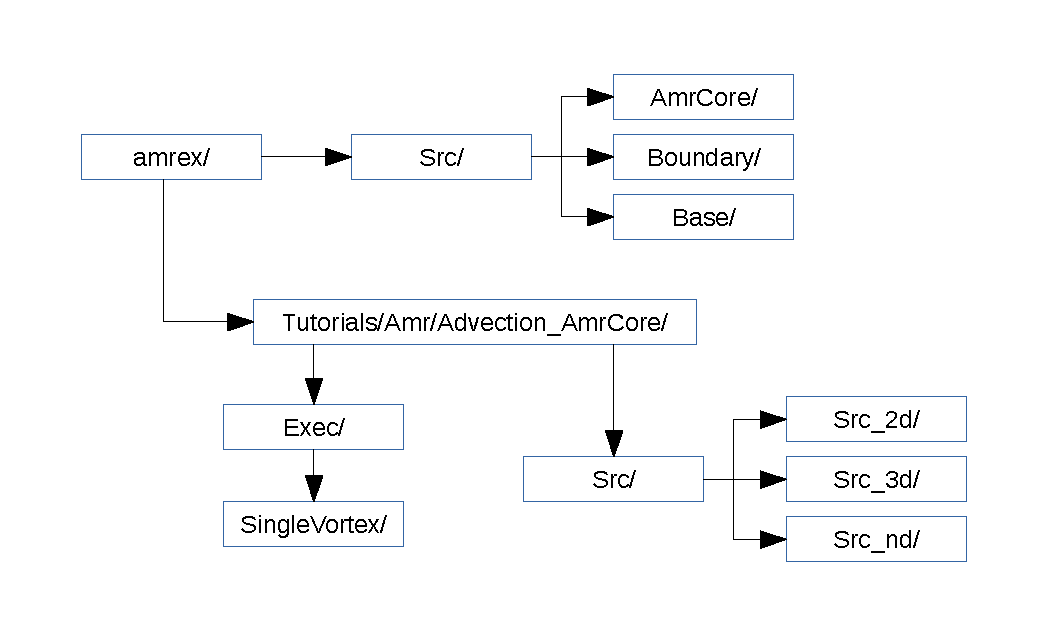
\includegraphics[width=4in]{./AmrCore/figs/flowchart.pdf}
\caption{\label{fig:AmrAdvection_AmrCore_flowchart} Source code tree for the 
         {\tt AmrAdvection\_AmrCore} example.}
\end{center}
\end{figure}
%%%%%%%%%%%%%%%%%%%%%%%%%%%%%
\begin{itemize}
\item {\tt amrex/Src/}
\begin{itemize}
\item {\tt Base/} Base {\tt amrex} library.
\item {\tt Boundary/} An assortment of classes for handling boundary data.
\item {\tt AmrCore/} AMR data management classes, described in more detail above.
\end{itemize}
\item {\tt Advection\_AmrCore/Src} Source code specific to this example.  Most notably
is the {\tt AmrCoreAdv} class, which is derived from {\tt AmrCore}.  The subdirectories {\tt Src\_2d}
and {\tt Src\_3d} contain dimension specific routines.  {\tt Src\_nd} contains dimension-independent routines.
\item {\tt Exec} Contains a makefile so a user can write other examples besides {\tt SingleVortex}.
\item {\tt SingleVortex} Build the code here by editing the {\tt GNUmakefile} and running {\tt make}.  There
is also problem-specific source code here used for initialization or specifying the velocity field used in this
simulation.
\end{itemize}

Here is a high-level pseudo-code of the flow of the program:
\begin{lstlisting}[language=cpp]
/* Advection_AmrCore Pseudocode */
main()
  AmrCoreAdv amr_core_adv; // build an AmrCoreAdv object
  amr_core_adv.InitData()  // initialize data all all levels
    AmrCore::InitFromScratch()
      AmrMesh::MakeNewGrids()
	AmrMesh::MakeBaseGrids() // define level 0 grids
	AmrCoreAdv::MakeNewLevelFromScratch()
          /* allocate phi_old, phi_new, t_new, and flux registers */
          initdata()  // fill phi
	if (max_level > 0) {
          do {
  	    AmrMesh::MakeNewGrids()
	      /* construct next finer grid based on tagging criteria */
 	    AmrCoreAdv::MakeNewLevelFromScratch()
              /* allocate phi_old, phi_new, t_new, and flux registers */
              initdata()  // fill phi
	  } (while (finest_level < max_level);
        }
  amr_core_adv.Evolve()
    loop over time steps {
      ComputeDt()
      timeStep() // advance a level
        /* check regrid conditions and regrid if necessary */
        Advance()
          /* copy phi into a multifab and fill ghost cells */
          /* advance phi */
          /* update flux registers */
        if (lev < finest_level) {
          timeStep() // recursive call to advance the next-finer level "r" times
            /* check regrid conditions and regrid if necessary */
            Advance()
              /* copy phi into a multifab and fill ghost cells */
              /* advance phi */
              /* update flux registers */
          reflux() // synchronize lev and lev+1 using fluxregister divergence
          AverageDown() // set covered coarse cells to be the average of fine
        }
    }
\end{lstlisting}

\subsection{The {\tt AmrCoreAdv} Class}
This example uses the class {\tt AmrCoreAdv}, which is derived from the class {\tt AmrCore} 
(which is derived from {\tt AmrMesh}).  The function definitions/implementations
are given in {\tt AmrCoreAdv.H/cpp}.

\subsection{{\tt FluxRegister}s}
The function {\tt AmrCoreAdv::Advance()} calls the fortran
subroutine, {\tt advect} (in {\tt ./Src\_xd/Adv\_xd.f90}).  {\tt advect} computes
and returns the time-advanced state as well as the fluxes used to update the state.
These fluxes are used to set or increment the flux registers.
\begin{lstlisting}[language=cpp]
// increment or decrement the flux registers by area and time-weighted fluxes
// Note that the fluxes have already been scaled by dt and area
// In this example we are solving phi_t = -div(+F)
// The fluxes contain, e.g., F_{i+1/2,j} = (phi*u)_{i+1/2,j}
// Keep this in mind when considering the different sign convention for updating
// the flux registers from the coarse or fine grid perspective
// NOTE: the flux register associated with flux_reg[lev] is associated
// with the lev/lev-1 interface (and has grid spacing associated with lev-1)
if (do_reflux) { 
   if (flux_reg[lev+1]) {
      for (int i = 0; i < BL_SPACEDIM; ++i) {
          flux_reg[lev+1]->CrseInit(fluxes[i],i,0,0,fluxes[i].nComp(), -1.0);
      }	    
   }
   if (flux_reg[lev]) {
      for (int i = 0; i < BL_SPACEDIM; ++i) {
          flux_reg[lev]->FineAdd(fluxes[i],i,0,0,fluxes[i].nComp(), 1.0);
      }
   }
}
\end{lstlisting}
The synchronization is performed at the end of {\tt AmrCoreAdv::timeStep}:
\begin{lstlisting}[language=cpp]
if (do_reflux)
{
    // update lev based on coarse-fine flux mismatch
    flux_reg[lev+1]->Reflux(*phi_new[lev], 1.0, 0, 0, phi_new[lev]->nComp(),
                            geom[lev]);
}

AverageDownTo(lev); // average lev+1 down to lev
\end{lstlisting}

\subsection{Regridding}
The {\tt regrid} function belongs to the {\tt AmrCore} class (it is virtual -- in this
tutorial we use the instance in {\tt AmrCore}).

At the beginning of each time step, we check whether we need to regrid.
In this example, we use a {\tt regrid\_int} and keep track of how many times each level
has been advanced.  When any given particular level $\ell<\ell_{\rm max}$ has been
advanced a multiple of {\tt regrid\_int}, we call the {\tt regrid} function.
\begin{lstlisting}[language=cpp]
void
AmrCoreAdv::timeStep (int lev, Real time, int iteration)
{
    if (regrid_int > 0)  // We may need to regrid
    {
        // regrid changes level "lev+1" so we don't regrid on max_level
        if (lev < max_level && istep[lev])
        {
            if (istep[lev] % regrid_int == 0)
            {
                // regrid could add newly refine levels
                // (if finest_level < max_level)
                // so we save the previous finest level index
		int old_finest = finest_level; 
		regrid(lev, time);

                // if there are newly created levels, set the time step
		for (int k = old_finest+1; k <= finest_level; ++k) {
		    dt[k] = dt[k-1] / MaxRefRatio(k-1);
		}
	    }
	}
    }
\end{lstlisting}

Central to the regridding process is the concept of ``tagging'' which cells need refinement.
{\tt ErrorEst} is a pure virtual function of {\tt AmrCore}, so each application code must
contain an implementation.  In {\tt AmrCoreAdv.cpp} the {\tt ErrorEst} function is essentially an
interface to a fortran routine that tags cells (in this case, {\tt state\_error} in 
{\tt Src\_nd/Tagging\_nd.f90}).  Note that this code uses tiling.
\begin{lstlisting}[language=cpp]
// tag all cells for refinement
// overrides the pure virtual function in AmrCore
void
AmrCoreAdv::ErrorEst (int lev, TagBoxArray& tags, Real time, int ngrow)
{
    static bool first = true;
    static Array<Real> phierr;

    // only do this during the first call to ErrorEst
    if (first)
    {
	first = false;
        // read in an array of "phierr", which is the tagging threshold
        // in this example, we tag values of "phi" which are greater than phierr
        // for that particular level
        // in subroutine state_error, you could use more elaborate tagging, such
        // as more advanced logical expressions, or gradients, etc.
	ParmParse pp("adv");
	int n = pp.countval("phierr");
	if (n > 0) {
	    pp.getarr("phierr", phierr, 0, n);
	}
    }

    if (lev >= phierr.size()) return;

    const int clearval = TagBox::CLEAR;
    const int   tagval = TagBox::SET;

    const Real* dx      = geom[lev].CellSize();
    const Real* prob_lo = geom[lev].ProbLo();

    const MultiFab& state = *phi_new[lev];

#ifdef _OPENMP
#pragma omp parallel
#endif
    {
        Array<int>  itags;
	
	for (MFIter mfi(state,true); mfi.isValid(); ++mfi)
	{
	    const Box& tilebox  = mfi.tilebox();

            TagBox&     tagfab  = tags[mfi];
	    
	    // We cannot pass tagfab to Fortran becuase it is BaseFab<char>.
	    // So we are going to get a temporary integer array.
            // set itags initially to 'untagged' everywhere
            // we define itags over the tilebox region
	    tagfab.get_itags(itags, tilebox);
	    
            // data pointer and index space
	    int*        tptr    = itags.dataPtr();
	    const int*  tlo     = tilebox.loVect();
	    const int*  thi     = tilebox.hiVect();

            // tag cells for refinement
	    state_error(tptr,  ARLIM_3D(tlo), ARLIM_3D(thi),
			BL_TO_FORTRAN_3D(state[mfi]),
			&tagval, &clearval, 
			ARLIM_3D(tilebox.loVect()), ARLIM_3D(tilebox.hiVect()), 
			ZFILL(dx), ZFILL(prob_lo), &time, &phierr[lev]);
	    //
	    // Now update the tags in the TagBox in the tilebox region
            // to be equal to itags
	    //
	    tagfab.tags_and_untags(itags, tilebox);
	}
    }
}
\end{lstlisting}
The {\tt state\_error} subroutine in {\tt Src\_nd/Tagging\_nd.f90} in this example
is simple:

\begin{lstlisting}[language=fortran]
subroutine state_error(tag,tag_lo,tag_hi, &
                       state,state_lo,state_hi, &
                       set,clear,&
                       lo,hi,&
                       dx,problo,time,phierr) bind(C, name="state_error")

  implicit none
  
  integer          :: lo(3),hi(3)
  integer          :: state_lo(3),state_hi(3)
  integer          :: tag_lo(3),tag_hi(3)
  double precision :: state(state_lo(1):state_hi(1), &
                            state_lo(2):state_hi(2), &
                            state_lo(3):state_hi(3))
  integer          :: tag(tag_lo(1):tag_hi(1), &
                          tag_lo(2):tag_hi(2), &
                          tag_lo(3):tag_hi(3))
  double precision :: problo(3),dx(3),time,phierr
  integer          :: set,clear

  integer          :: i, j, k

  ! Tag on regions of high phi
  do       k = lo(3), hi(3)
     do    j = lo(2), hi(2)
        do i = lo(1), hi(1)
           if (state(i,j,k) .ge. phierr) then
              tag(i,j,k) = set
           endif
        enddo
     enddo
  enddo

end subroutine state_error
\end{lstlisting}

\subsection{FillPatch}
This example has two functions, {\tt AmrCoreAdv::FillPatch} and {\tt AmrCoreAdv::CoarseFillPatch},
that make use of functions in {\tt AmrCore/AMReX\_FillPatchUtil}.

In {\tt AmrCoreAdv::Advance}, we create a temporary {\tt MultiFab} called {\tt Sborder}, which
is essentially $\phi$ but with ghost cells filled in.  The valid and ghost cells are filled in from
actual valid data at that level, space-time interpolated data from the next-coarser level, 
neighboring grids at the same level, or domain boundary conditions 
(for examples that have non-periodic boundary conditions).
\begin{lstlisting}[language=cpp]
MultiFab Sborder(grids[lev], dmap[lev], S_new.nComp(), num_grow);
FillPatch(lev, time, Sborder, 0, Sborder.nComp());
\end{lstlisting}
Several other calls to fillpatch routines are hidden from the user in the regridding process.
